\subsection{Evaluating the forces using the Fast Multipole Method}
\label{ssec:fmm_summary}

The algorithmically challenging aspect of the \nbody problem is to
evaluate for each particle in a system the potential and associated
forces generated by all the other particles. Mathematically, this means
evaluate
\begin{equation}
  \phi(\mathbf{x}_a) = \sum_{b \neq a} G m_b\varphi(\mathbf{x}_a -
  \mathbf{x}_b)\qquad \forall~a\in N
  \label{eq:fmm:n_body}
\end{equation}
efficiently for large numbers of particles $N$. In the case of
collisionless dynamics, the particles are a mere Monte-Carlo sampling
of the underlying coarse-grained phase-space distribution which
justifies the use of approximate method to evaluate
Eq.~\ref{eq:fmm:n_body}. The \emph{Fast Multipole Method} (FMM)
\citep{Greengard1987, Cheng1999}, popularized in astronomy and adapted
specifically for gravity solvers by \cite{Dehnen2000, Dehnen2002} (see
also \cite{Warren1995} for related ideas), is an $\mathcal{O}(N)$
method designed to solve Eq.~\ref{eq:fmm:n_body} by expanding the
potential in Taylor series \emph{both} around $\mathbf{x}_a$ and
$\mathbf{x}_b$ and grouping similar terms arising from nearby
particles. For comparison, a \cite{Barnes1986} tree-code expands the
potential only around $\mathbf{x}_b$.

\subsubsection{Double expansion of the potential}

\begin{figure}
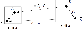
\includegraphics[width=\columnwidth]{cells.pdf}
\caption{The basics of the FMM: The potential generated by a particle
  at position $\mathbf{x}_b$ on a particle at position at location
  $\mathbf{x}_a$ is replaced by a Taylor expansion of the potential
  around the distance vector $\mathbf{R}$ linking the two centres of mass
  ($\mathbf{z}_A$ and $\mathbf{z}_B$) of cell $A$ and $B$. The
  expansion converges towards the exact expression provided
  $|\mathbf{R}|>|\mathbf{r}_a + \mathbf{r}_b|$.}
\label{fig:fmm:cells}
\end{figure}

In what follows, we use the compact multi-index notation of
\cite{Dehnen2014} (repeated in appendix \ref{sec:multi_index_notation}
for completeness) to simplify expressions and ease comparisons with
other published work. $\mathbf{k}$, $\mathbf{m}$ and $\mathbf{n}$ are
multi-indices and $\mathbf{r}$, $\mathbf{R}$, $\mathbf{x}$,
$\mathbf{y}$ and $\mathbf{z}$ are vectors, whilst $a$ and $b$ are
particle indices. Note also that we make no assumption on the specific
functional form of the potential $\varphi$.\\
For a single pair of particles $a$ and $b$ located in cell $A$ and $B$
with centres of mass $\mathbf{z}_A$ and $\mathbf{z}_B$ respectively,
as shown on Fig.~\ref{fig:fmm:cells}, the potential generated by $b$
at the location of $a$ can be rewritten as
\begin{align}
  \varphi(\mathbf{x}_a - \mathbf{x}_b)
  &= \varphi\left(\mathbf{x}_a - \mathbf{z}_A - \mathbf{x}_b +
  \mathbf{z}_B + \mathbf{z}_A - \mathbf{z}_B\right)  \nonumber \\
  &= \varphi\left(\mathbf{r}_a - \mathbf{r}_b + \mathbf{R}\right)
  \nonumber \\
  &= \sum_\mathbf{k} \frac{1}{\mathbf{k}!} \left(\mathbf{r}_a -
  \mathbf{r}_b\right)^{\mathbf{k}} \nabla^{\mathbf{k}}\varphi(\mathbf{R})
  \nonumber \\
  &= \sum_\mathbf{k} \frac{1}{\mathbf{k}!} \sum_{\mathbf{n} <
    \mathbf{k}} \binom{\mathbf{k}}{\mathbf{n}} \mathbf{r}_a^{\mathbf{n}}
  \left(-\mathbf{r}_b\right)^{\mathbf{k} - \mathbf{n}}
  \nabla^{\mathbf{k}}\varphi(\mathbf{R})\nonumber \\
  &= \sum_\mathbf{n} \frac{1}{\mathbf{n}!} \mathbf{r}_a^{\mathbf{n}}
  \sum_\mathbf{m} \frac{1}{\mathbf{m}!}
  \left(-\mathbf{r}_b\right)^\mathbf{m} \nabla^{\mathbf{n}+\mathbf{m}} \varphi(\mathbf{R}),
  \label{eq:fmm:expansion}
\end{align}
where we used the Taylor expansion of $\varphi$ around $\mathbf{R} \equiv
\mathbf{z}_A - \mathbf{z}_B$ on the third line, used $\mathbf{r}_a
\equiv \mathbf{x}_a - \mathbf{z}_A$, $\mathbf{r}_b \equiv \mathbf{x}_b
- \mathbf{z}_B$ throughout and defined $\mathbf{m} \equiv
\mathbf{k}-\mathbf{n}$ on the last line. Expanding the series only up
to order $p$, we get
\begin{equation}
  \varphi(\mathbf{x}_a - \mathbf{x}_b) \approx \sum_{\mathbf{n}}^{p}
  \frac{1}{\mathbf{n}!} \mathbf{r}_a^{\mathbf{n}} \sum_{\mathbf{m}}^{p
    -|\mathbf{n}|} 
  \frac{1}{\mathbf{m}!} \left(-\mathbf{r}_b\right)^\mathbf{m}
  \nabla^{\mathbf{n}+\mathbf{m}} \varphi(\mathbf{R}),
  \label{eq:fmm:fmm_one_part}
\end{equation}
with the approximation converging as $p\rightarrow\infty$ towards the
correct value provided $|\mathbf{R}|>|\mathbf{r}_a +
\mathbf{r}_b|$. If we now consider all the particles within $B$ and
combine their contributions to the potential at location
$\mathbf{x}_a$ in cell $A$, we get
\begin{align}
  \phi_{BA}(\mathbf{x}_a) &= \sum_{b\in B}G m_b\varphi(\mathbf{x}_a -
  \mathbf{x}_b)  \label{eq:fmm:fmm_one_cell}  \\
  &\approx G\sum_{\mathbf{n}}^{p}
  \frac{1}{\mathbf{n}!} \mathbf{r}_a^{\mathbf{n}} \sum_{\mathbf{m}}
    ^{p -|\mathbf{n}|}
  \frac{1}{\mathbf{m}!} \sum_{b\in B} m_b\left(-\mathbf{r}_b\right)^\mathbf{m}
  \nabla^{\mathbf{n}+\mathbf{m}} \varphi(\mathbf{R}) \nonumber. 
\end{align}
This last equation forms the basis of the FMM. The algorithm
decomposes the equation into three separated sums evaluated at
different stages.\\

\subsubsection{The FMM algorithm}

In a first step, multipoles are constructed from the
innermost sum. For each cell, we compute all the terms
\begin{equation}
  \mathsf{M}_{\mathbf{m}}(\mathbf{z}_B) = \frac{1}{\mathbf{m}!}
  \sum_{b\in B} m_b\left(-\mathbf{r}_b\right)^\mathbf{m} \label{eq:fmm:P2M} 
\end{equation}
up to order $p$. This is the first kernel of the method, commonly
labelled as \textsc{P2M} (particle to multipole). In a second step, we
compute the second kernel, \textsc{M2L} (multipole to local
expansion), which corresponds to the interaction of a cell with
another one:
\begin{equation}
  \mathsf{F}_{\mathbf{n}}(\mathbf{z}_A) = G\sum_{\mathbf{m}}^{p -|\mathbf{n}|}
  \mathsf{M}_{\mathbf{m}}(\mathbf{z}_B)
  \mathsf{D}_{\mathbf{n}+\mathbf{m}}(\mathbf{R}), \label{eq:fmm:M2L} 
\end{equation}
where $\mathsf{D}_{\mathbf{n}+\mathbf{m}}(\mathbf{R}) \equiv
\nabla^{\mathbf{n}+\mathbf{m}} \varphi(\mathbf{R})$ is an order $n+m$
derivative of the potential. This is the computationally expensive
step of the FMM algorithm as the number of operations in a naive
implementation using cartesian coordinates scales as
$\mathcal{O}(p^6)$. More advanced techniques
\citep[e.g.][]{Dehnen2014} can bring the cost down to
$\mathcal{O}(p^3)$, albeit at a considerable algebraic cost. For
collisionless dynamics, high accuracy is not required and low values
of $p$ are sufficient, which maintains the computational cost of the
M2L kernel at a reasonable level.  
Finally, in the last step, the potential is propagated from the local
expansion centre to the particles (L2P kernel) using
\begin{equation}
  \phi_{BA}(\mathbf{x}_a) = \sum_{\mathbf{n}}^{p}
  \frac{1}{\mathbf{n}!} \mathbf{r}_a^{\mathbf{n}}
  \mathsf{F}_{\mathbf{n}}(\mathbf{z}_A). \label{eq:fmm:L2P} 
\end{equation}
In summary, the potential generated by a cell $B$ on the particles in
cell $A$ is obtained by the successive application of the P2M, M2L and
L2P kernels. The P2M and L2P kernels are applied only once per
particle, whilst one M2L calculation has to be performed for each pair
of cells. The forces applied to the particles are obtained by the same
procedure using an extra order in the Taylor expansion. For instance,
for the acceleration along $x$, we have:
\begin{equation}
  a_x(\mathbf{x}_a) = \sum_{\mathbf{n}}^{p-1}
  \frac{1}{\mathbf{n}!} \mathbf{r}_a^{\mathbf{n}}
  \mathsf{F}_{\mathbf{n}+\left(1,0,0\right)}(\mathbf{z}_A). \label{eq:fmm:L2P_force} 
\end{equation}
In practice, the multipoles can be constructed recursively from the
leaves of the tree to the root and the local expansions from the root
to the leaves by shifting the $\mathsf{M}$ and $\mathsf{F}$ tensors
and adding their contributions to their parent or daughter cell's
tensors respecitvely. The shifting formulas (M2M and L2L kernels)
read:

\begin{align}
  \mathsf{M}_{\mathbf{m}}(\mathbf{x} + \mathbf{y}) &=
  \sum_{\mathbf{n}}^{\mathbf{m}}
  \frac{\mathbf{y}^\mathbf{n}}{\mathbf{n}!}\mathsf{M}_{\mathbf{m} -
    \mathbf{n}}(\mathbf{x}), \label{eq:fmm:M2M} \\
  \mathsf{F}_{\mathbf{n}}(\mathbf{x} + \mathbf{y}) &=
  \sum_{\mathbf{m}}^{p-|\mathbf{n}|}
  \frac{\mathbf{y}^\mathbf{m}}{\mathbf{m}!}\mathsf{F}_{\mathbf{m} +
    \mathbf{n}}(\mathbf{x}). \label{eq:fmm:L2L} 
\end{align}
One final, useful expression that enters some interaction between
tree-leaves is the P2M kernel that directly applies the potential due
to a multipole expansion to a particle without using the expansion of
the potential $\mathsf{F}$ at the centre of mass of the cell. This
kernel is obtained by setting $\mathbf{r}_a$ to zero in
eq.~\ref{eq:fmm:expansion}, re-defining
$\mathbf{R}\equiv\mathbf{x}_{\rm a} - \mathbf{z}_{\rm B}$ and
constructing the same $\mathsf{M}$ and $\mathsf{D}$ tensor than for
the other kernels:
\begin{align}
  \phi_{Ba}(\mathbf{x}_a) &= G\sum_{\mathbf{m}}^p \mathsf{M}_{\mathbf{m}} \mathsf{D}_{\mathbf{m}}(\mathbf{R}),\\
  a_x(\mathbf{x}_a) &= G\sum_{\mathbf{m}}^p \mathsf{M}_{\mathbf{m}} \mathsf{D}_{\mathbf{m}+\left(1,0,0\right)}(\mathbf{R}).
  \label{eq:fmm:M2P}
\end{align}
A traditional tree-code uses solely that kernel to obtain the forces
from the multipoles (or often just monopoles, i.e. setting $p=0$ throughout)
to the particles.\\
All the kernels (Eqs.~\ref{eq:fmm:P2M}-\ref{eq:fmm:M2P}) are rather
straightforward to evaluate as they are only made of additions and
multiplications (provided $\mathsf{D}$ can be evaluated quickly),
which are extremely efficient instructions on modern architectures
(see Appendix \ref{sec:pot_derivatives} for the full
expressions). However, the fully expanded sums can lead to rather
large and prone to typo expressions. To avoid any mishaps, we use a
\texttt{python} script to generate C code in which all the sums are
unrolled and correct by construction. In \swift, we implemented the
kernels up to order $p=5$, as it proved to be accurate enough for our
purpose, but this could be extended to higher order easily. This
implies storing $56$ numbers per cell for each $\textsf{M}$ and
$\textsf{F}$ plus three numbers for the location of the centre of
mass. For leaf-cells with large numbers of particles, as in \swift,
this is a small memory overhead. One further small improvement
consists in choosing $\mathbf{z}_A$ to be the centre of mass of cell
$A$ rather than its geometrical centre. The first order multipoles
($\mathsf{M}_{100},\mathsf{M}_{010},\mathsf{M}_{001}$) then vanish by
construction. This allows us to simplify some of the expressions and
helps reduce, albeit by a small fraction, the memory footprint of the
tree structure.

\subsubsection{Computing the accelerations via a tree-walk}

We define the maximal distance between a centre of mass of a cell $B$ and
any particle in that cell as

\begin{equation}
  \rho_B = \max_{b \in B}(|\mathbf{r}_b|)
\end{equation}
\\
\textcolor{red}{MORE WORDS HERE}

\subsubsection{The multipole acceptance criterion}

The main remaining question is to decide when two cells are far enough from
each others that the truncated Taylor expansion used as approximation for
the potential (eq. \ref{eq:fmm:expansion}) is accurate enough. The
criterion used to make that decision is called the \emph{multipole
  acceptance criterion} (MAC).

We know that (\ref{eq:fmm:expansion}) is converging towards the correct
answer provided $1>|\mathbf{r}_a + \mathbf{r}_b| / |\mathbf{R}|$. This is
hence the most basic (and always necessary) MAC that can be designed. If
this ratio is lower, the accuracy (at a fixed expansion order) is improved
and it is hence common practice to define a critical \emph{opening angle}
$\theta_{\rm cr}$ and allow the use of the multipole approximation between
two cells if

\begin{equation}
  \theta_{\rm cr} > \frac{\rho_A + \rho_B} {|\mathbf{R}|}.
  \label{eq:fmm:angle}
\end{equation}
This lets users have a second handle on the accuracy on the gravity
calculation besides the much more involved change in the expansion order
$p$ of the FMM method. Typical values for the opening angle are in the
range $[0.3, 0.7]$, with the cost of the simulation growing as $\theta_{\rm
  cr}$ decreases.

This method has the drawback of using a uniform criterion across the entire
simulation volume and time evolution, which means that the chosen value of
$\theta_{\rm cr}$ could be too small in some regions (leading to too many
operations for the expected accuracy) and too large in some other other
ones (leading to a lower level of accuracy than expected). \swift instead
uses a more adaptive criterion to decide when the multipole approximation
can be used. This is based on the error analysis of FMM by
\cite{Dehnen2014} and is summarised below for completeness. The key idea is
to exploit the additional information about the distribution of particles
that is encoded in the higher-order multipole terms.

We start by defining the scalar quantity $\mathsf{P}_{A,n}$, the
\emph{power} of the multipole of order $n$ of the particles in cell $A$,
via
\begin{equation}
  \mathsf{P}_{A,n}^2 = \sum_{|\mathbf{m}|=n} \frac{\mathbf{m}!}{|\mathbf{m}|!}\mathsf{M}_{A,\mathbf{m}}^2,
\end{equation}
where the sum runs over all the multipole terms of order $n$ in the
cell\footnote{Note that $\mathsf{P}_{0} \equiv \mathsf{M}_{(0,0,0)}$ is
  just the mass of the cell and since \swift uses the centre of mass as the
  centre of expansion of the multipoles, $\mathsf{P}_{1} = 0$.}. This
quantity is a simple upper bound for the amplitude of the multipole
($\mathsf{M}_{A, \mathbf{m}} < \mathsf{P}_{A,|\mathbf{m}|}/|\mathbf{m}|!$)
and can hence be used to estimate the importance of the terms of a given
order in the Taylor series of the potential. Following \cite{Dehnen2014} we
then consider a source cell $A$ and a sink cell $B$ for which we evaluate
at order $p$ the expression
\begin{equation}
  E_{AB} = \frac{1}{M_A|\mathbf{R}|^p} \sum_m^p \binom{p}{m} \mathsf{P}_m
  \rho_B^{p-m},
  \label{eq:fmm:e_ab}
\end{equation}
with $M_A \equiv \mathsf{M}_{A,(0,0,0)}$, the sum of the mass of the
particles in the cell. Note that since $\mathsf{P}_{A,n} \leq M_A
\rho_A^n$, we have $E_{AB} \leq \left((\rho_A +
\rho_B)/|\mathbf{R}|\right)^p$, where the right-hand side is the expression
used in the basic opening angle condition (\ref{eq:fmm:angle}). We finally
scale the $E_{AB}$'s by the relative size of the two cells to define the
error estimator $\tilde{E}_{AB}$:
\begin{equation}
  \tilde{E}_{AB} = 8\frac{\max(\rho_A, \rho_B)}{\rho_A + \rho_B}E_{AB}.
  \label{eq:fmm:e_ab_tilde}
\end{equation}
As shown by \cite{Dehnen2014}, these quantities are excellent estimators of
the error made in computing the accelerations between two cells using the
M2L and M2P kernels at a given order. We can hence use this property to
design a new MAC by demanding that the estimated acceleration error is no
larger than a certain fraction of the smallest acceleration in the sink
cell $B$. This means we can use the FMM approximation between to
approximate the accelerations in cell $A$ due to the particles in cell $B$ if
\begin{equation}
  \tilde{E}_{AB} \frac{M_A}{|\mathbf{R}|^2} < \epsilon \min_{b\in
    B}\left(|\mathbf{a}_b|\right) \quad \rm{and} \quad \frac{\rho_A +
    \rho_B} {|\mathbf{R}|} < 1,
  \label{eq:fmm:mac}  
\end{equation}
where the $\mathbf{a}_b$ are the accelerations of the particles in cell $B$
and $\epsilon$ is a tolerance parameter. Since this is self-referencing
(i.e. we need the accelerations to decide how to compute the
accelerations), we need to use a an estimator of $|\mathbf{a}_b|$. In
\swift, we follow the strategy used by \gadget and use the acceleration of
the previous time-step\footnote{On the first time-step of a simulation this
  value has not been computed yet. We hence run a fake 0th time-step with
  the simpler MAC (eq. \ref{eq:fmm:angle}), which is good enough to obtain
  approximations of the accelerations.}. The minimal norm of the
acceleration in a given cell can be computed at the same time as the P2M
and M2M kernels are evaluated in the tree construction phase. The second
condition in (\ref{eq:fmm:mac}) is necessary to ensure the convergence of the
Taylor expansion.

In the specific case of the M2P kernel, we have $\rho_B = 0$, which
simplifies some of the expressions above. In this case, at order $p$, we get:
\begin{align}
  E_{AB} &= \frac{\mathsf{P}_{p, A}}{M_A |\mathbf{R}|^p}, \nonumber \\
  \tilde{E}_{AB} &= 8E_{AB} \nonumber 
\end{align}
This leads to the following MAC for the M2P kernel:
\begin{equation}
  8\frac{\mathsf{P}_{p, A}}{|\mathbf{R}|^{p+2}} < \epsilon \min_{b\in
    B}\left(|\mathbf{a}_b|\right) \quad \rm{and} \quad \frac{\rho_A}
  {|\mathbf{R}|} < 1.
    \label{eq:fmm:mac_m2p}  
\end{equation}
The value of $\epsilon$ could in principle be different than the one
used for the M2L MAC. One specific case is of particular
interest. Using the expression for order $2$ and the approximation
$P_{A,p} \approx M_A \rho_A^p$, we get
\begin{equation}
  8\frac{M_A}{|\mathbf{R}|^2}\left(\frac{\rho_A}{|\mathbf{R}|}\right)^2
  < \epsilon \min_{b\in B}\left(|\mathbf{a}_b|\right) \nonumber
\end{equation}
for our MAC.  This is the same expression as the adaptive opening
angle used by \gadget \cite[see eq.18 of][]{Springel2005} up to
numerical factors and definition of the size ($\rho$ vs. the cell
edge) of a multipole. Note, however, that, in practice, since formally
$P_{A,p} \leq M_A \rho_A^p$, the dependence is slightly different.

